\subsection{Fukuda's algorihm}

%vague overview
Fukuda's algorithm allows to enumerate all the vertices of an $\mathcal{H}$-polytope included in the positive orthant ($(\mathbb{R}_+)^d$, all its points have non-negative coordinates) and with the origin as a vertex. This algorithm uses the pivoting scheme of the simplex to explore the polytope. 

It is based on a simple idea: starting from any vertex, the simplex algorithm allows to reach a vertex maximizing a linear function by a unique (thanks to Bland's rule) path among the vertices. The algorithm picks a function maximized only by the origin on the positive orthant and walks backward on all the paths leading to it from all the vertices. Every time a vertex is encountered, it is output.

The first thing to do is to find the end of all these paths: the dictionary corresponding to the origin. It consists in taking the canonical base as cobasis and the set constraints as the basis and setting $-\sum_{i=0}^d x_i$ as the cost function. All the possible pivots are tried from this dictionary. If a pivot leads to a primal feasible dictionary (defining a vertex of the polytope) for which the Bland's method leads back to the previous point it is said to be a valid reverse Bland's pivot. It means that a step backward has been made on one of the paths, the new point is output, and the method has to be applied from this new point.

However, if a vertex is defined by more hyperplanes than required, several dictionaries will describe the same point, which is said to be degenerated. Fukuda overcomes this problem by defining a partial order on the dictionaries. This order corresponds to a lexicographic order on the basis for the dictionaries defining the same point. A point is only output if its dictionary is lexicographical minimal. Note that the algorithm continues on the dictionary, even if it is not lexicographical minimal. A dictionary which is not lexicographical minimal might still be one the path of an other vertex to reach the origin.


If the origin is degenerated, then all the optimal dictionaries defining it have to be found. This is done by using a procedure very similar from the one above: by looking only at the hyperplanes redefining the origin, every pivot is tried. The difference is instead of using the Bland's rule, a variation of the dual Bland's rule is used. If the new dictionary is dual feasible (still an optimal for the cost function) and the dual Bland's rule brings it back to the previous one, then the new dictionary is valid with respect to the dual Bland's rule etc. This research presents the same uniqueness properties than the previous one. The previous research has to be launched from every dictionary obtained this way.

Figure~\ref{ex_fuku} shows the paths to reach the origin for the vertices of the unit cube (constraints: $0\leq x,y,z \leq 1$) and the tree of the exploration made by the algorithm.

\vspace*{-1cm}

\begin{figure}
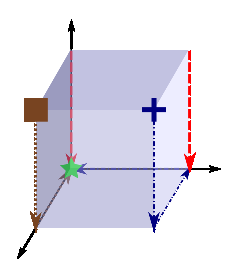
\includegraphics[scale=1.1]{images/fukuda.eps}
\hspace*{0.5cm}
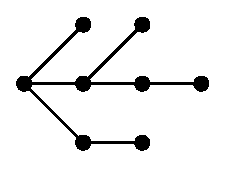
\includegraphics[scale=1]{images/fukugraph.eps}
\caption{On the left:  the paths to reach the origin for the vertices of the unit cube (constraints: $0\leq x,y,z \leq 1$). On the right: the tree of the vertices given by Fukuda's algorithm. Its nodes corresponds to the vertices, its edges are the paths and its root corresponds to the origin.}
\label{ex_fuku}
\end{figure}

\paragraph{Complexity:} for $n$ half-space in a space of dimension $d$, Fukuda gives a complexity of $O(nd(n+d)g)$, where $g$ is the number of vertices of the polyhedron, counted with their multiplicity (a degenerated vertex can be define in several ways, it is counted several times). 
